\documentclass{dclass}
\usepackage{hyperref}
\hypersetup{
colorlinks=true,
urlcolor=blue,
citecolor=blue}
\usepackage[all]{xy,xypic}
\usepackage{amsfonts,amssymb,amsmath,amsgen,amsopn,amsbsy,theorem,graphicx,epsfig}
\usepackage{eufrak,amscd,bezier,latexsym,mathrsfs,eurosym,enumerate}
\usepackage[utf8]{inputenc}
\usepackage[english]{babel}
\usepackage{cleveref,multirow}
\usepackage[dvipsnames]{xcolor}
\usepackage[pagewise]{lineno}
\usepackage{listings}
\usepackage{array}


\title{Rust and Go Programming Languages}

\author[YASSER AL HASAN and HARUN ADEM TEMUR]{
\textbf{YASSER AL HASAN$^{1}$, HARUN ADEM TEMUR$^{2}$}\\
$^{1}$Department of Computer Engineering, Faculty of Engineering, Dokuz Eylül University, İzmir, Turkey. \\
$^{2}$Department of Computer Engineering, Faculty of Engineering, Dokuz Eylül University, İzmir, Turkey. \\
\\ [1.8em]

\date{May 18, 2023}

}

\def\E{\ifmmode{\mathbb E}\else{$\mathbb E$}\fi} %natural numbers
\def\N{\ifmmode{\mathbb N}\else{$\mathbb N$}\fi} %natural numbers
\def\R{\ifmmode{\mathbb R}\else{$\mathbb R$}\fi} %real numbers
\def\Q{\ifmmode{\mathbb Q}\else{$\mathbb Q$}\fi} %rational numbers
\def\C{\ifmmode{\mathbb C}\else{$\mathbb C$}\fi} %complex numbers
\def\H{\ifmmode{\mathbb H}\else{$\mathbb H$}\fi} %complex numbers
\def\Z{\ifmmode{\mathbb Z}\else{$\mathbb Z$}\fi} %integers
\def\P{\ifmmode{\mathbb P}\else{$\mathbb P$}\fi} %real numbers
\def\T{\ifmmode{\mathbb T}\else{$\mathbb T$}\fi} %real numbers
\def\SS{\ifmmode{\mathbb S}\else{$\mathbb S$}\fi} %real numbers
\def\DD{\ifmmode{\mathbb D}\else{$\mathbb D$}\fi} %real numbers

\renewcommand{\a}{\alpha}
\renewcommand{\b}{\beta}
\renewcommand{\d}{\delta}
\newcommand{\D}{\Delta}
\newcommand{\e}{\epsilon}
\newcommand{\var}{\varepsilon}
\newcommand{\g}{\gamma}
\newcommand{\la}{\lambda}
\newcommand{\La}{\Lambda}
\newcommand{\lan}{\langle}
\newcommand{\ran}{\rangle}
\newcommand{\n}{\nabla}
\newcommand{\va}{\varphi}
\newcommand{\s}{\sigma}
\newcommand{\Sig}{\Sigma}
\renewcommand{\t}{\tau}
\renewcommand{\th}{\theta}
\newcommand{\Om}{\Omega}
\newcommand{\om}{\omega}
\newcommand{\pa}{\partial}
\newcommand{\up}{\upsilon}
\newcommand{\vp}{\varphi}
\newcommand{\z}{\zeta}





\newcommand{\bse}{\begin{subequations}}
\newcommand{\ese}{\end{subequations}}
\newcommand{\ben}{\begin{enumerate}}
\newcommand{\een}{\end{enumerate}}
\newcommand{\bens}{\begin{enumerate*}}
\newcommand{\eens}{\end{enumerate*}}
\newcommand{\be}{\begin{equation}}
\newcommand{\ee}{\end{equation}}
\newcommand{\bea}{\begin{eqnarray}}
\newcommand{\eea}{\end{eqnarray}}
\newcommand{\baa}{\begin{eqnarray*}}
\newcommand{\eaa}{\end{eqnarray*}}
\newcommand{\bc}{\begin{center}}
\newcommand{\ec}{\end{center}}
\newcommand{\ol}{\overline}
\newcommand{\ul}{\underline}
\newcommand{\ov}{\overbrace}
\newcommand{\uv}{\underbrace}
\newcommand{\Ra}{\Rightarrow}
\newcommand{\ra}{\rightarrow}
\newcommand{\ds}{\displaystyle}
\newcommand{\vs}{\vspace}


\newcommand{\IR}{\mbox{I \hspace{-0.2cm}R}}
\newcommand{\IN}{\mbox{I \hspace{-0.2cm}N}}



%% \theoremstyle{plain} %% This is the default

\newtheorem{theorem}{Theorem}%[section]

\theoremstyle{corollary}
\newtheorem{corollary}{Corollary}

\theoremstyle{lemma}
\newtheorem{lemma}{Lemma}

\theoremstyle{proposition}
\newtheorem{proposition}{Proposition}

\theoremstyle{axiom}
\newtheorem{axiom}{Axiom}

\theoremstyle{conjecture}
\newtheorem{conjecture}{Conjecture}

\theoremstyle{example}
\newtheorem{example}{Example}

\theoremstyle{definition}
\newtheorem{definition}{Definition}%[section]

\theoremstyle{remark}
\newtheorem{remark}{Remark}%[section]
\newtheorem{notation}{Notation}


\newtheorem{question}{Question}%[section]
\newtheorem{construction}{Construction}

\newtheorem{athm}{Theorem}
\renewcommand{\theathm}{\Alph{athm}}





\setcounter{page}{1}
\begin{document}

\maketitle


\begin{abstract}In this report, we will provide an in-depth comparison of Go and Rust. We will discuss their similarities and differences, and provide examples of how they can be used to solve different problems. We will also compare their variables, conditions, loops, and subprograms, and provide recommendations for which language to use for different types of projects. By the end of this report, you will have a better understanding of the strengths and weaknesses of Go and Rust, and be able to choose the language that best fits your needs.

\end{abstract}

\section{Introduction}
\label{Int}

In recent years, the software development industry has seen a surge in the popularity of modern programming languages such as Go and Rust. These languages have been designed to be fast, efficient, and reliable, with a focus on concurrency and parallelism. Go, in particular, has gained a lot of attention in the cloud computing industry because of its ability to handle large-scale distributed systems. Rust, on the other hand, has become popular in the systems programming community due to its advanced memory safety and thread safety features.
Both Go and Rust offer unique features and capabilities that make them ideal for different types of projects. Go is a general-purpose language that is well-suited for web development, systems programming, and cloud computing. It has a simple syntax, making it easy to learn and use, and offers automatic memory management, which makes it easier to write and maintain code. \cite{ref1}Rust, on the other hand, is a systems programming language that is designed for low-level programming and memory safety. It offers a unique ownership and borrowing system, which helps prevent common memory-related issues such as data races and null pointer errors.

\section{Overview of both languages}
\subsection{Go}

Go is a modern, open-source programming language that was developed by a team at Google, led by Rob Pike and Ken Thompson, in 2007. The language was designed to be fast, efficient, and easy to use, with a focus on concurrency and parallelism. Go is a statically typed language that is compiled, making it faster and more efficient than interpreted languages such as Python or Ruby.\\\\
Go is a general-purpose language that can be used for a wide range of applications, including web development, systems programming, and network programming. It has a simple syntax that is easy to learn, making it a good choice for beginners. Go also has a garbage collector, which makes memory management easier, and it supports multi-threading and network programming out of the box.\\\\
Go's built-in support for concurrency and parallelism is one of its key strengths. This makes it well-suited for developing high-performance software systems that can handle large-scale distributed systems. Go's popularity has grown in recent years due to its use in cloud computing, where it is used to build scalable, distributed systems.\\
\subsection{Rust}
Rust is a modern, open-source systems programming language that was developed by Mozilla in 2010. The language was designed to provide a safer alternative to C and C++, with a focus on memory safety and thread safety. Rust is a statically typed language that is compiled, making it fast and efficient.\cite{ref2}\\\\
Rust's unique feature is its ownership and borrowing system, which ensures that only one part of the code can access a particular piece of data at a time, preventing data races and other memory-related issues. Rust's focus on memory safety and thread safety has made it a popular choice for developing low-level systems, such as operating systems, device drivers, and game engines.\\\\
Rust's syntax is more complex than Go's, which can make it more difficult to learn for beginners. However, Rust's advanced memory safety features make it a good choice for developing software systems that require high levels of security and reliability.\\\\
In addition to its memory safety features, Rust also has a powerful macro system and a package manager called Cargo, which makes it easy to manage dependencies and build projects. Rust also has a growing ecosystem of libraries and tools, making it easier to get started with the language.\\\\\\
Overall, both Go and Rust are powerful programming languages that offer unique features and capabilities. They are both fast, efficient, and reliable, and are ideal for different types of projects. Go is a general-purpose language that is well-suited for web development, systems programming, and cloud computing, while Rust is a systems programming language that is well-suited for low-level programming and memory safety. The choice between the two languages will depend on the specific needs and requirements of the project.\\
\subsection{Main differences between the two languages}

\begin{table}[h!]
\centering
\vspace{0.2cm}
\begin{tabular}{|l|c|c|}
\hline
\textbf{Characteristics} & \textbf{Go} & \textbf{Rust} \\
\hline
Memory Management & Garbage collected & Ownership model with compiler checks \\
\hline
Speed \& Performance & Medium & High \\
\hline
Difficulty to learn & Low & High \\
\hline
Compile time & Fast & Slow \\
\hline
Deployment & Static Binary & Static Binary \\
\hline
Concurrency & Goroutines & Async/await \& threading \\
\hline
Use on embedded devices & Narrow & Broad \\
\hline
\end{tabular}
\caption{Comparison of Go and Rust}
\label{tab:comparison}
\end{table}

\subsection{Security of Go and Rust}

Go and Rust are both modern programming languages that prioritize memory safety. Rust is designed to provide low-level control over system resources and memory, similar to languages like C and C++. It achieves high performance through zero-cost abstractions, which means that the abstractions have little to no runtime overhead. This allows developers to write high-level code without sacrificing performance. Rust’s heavy emphasis on preventing memory-related security vulnerabilities means programmers have to go out of their way to perform tasks that would be simpler in other languages, including Go.\\\\
Go (also known as Golang) was designed by Google engineers who wanted a language that offered the efficiency of C++, but was easier to learn, write, read, and deploy. The language’s “Goroutines” make it easy for developers to build applications that take full advantage of concurrency. Go prioritizes simplicity and ease of use, making it an attractive option for large-scale back-end systems and infrastructure.

\begin{figure}[h!]
\begin{center}
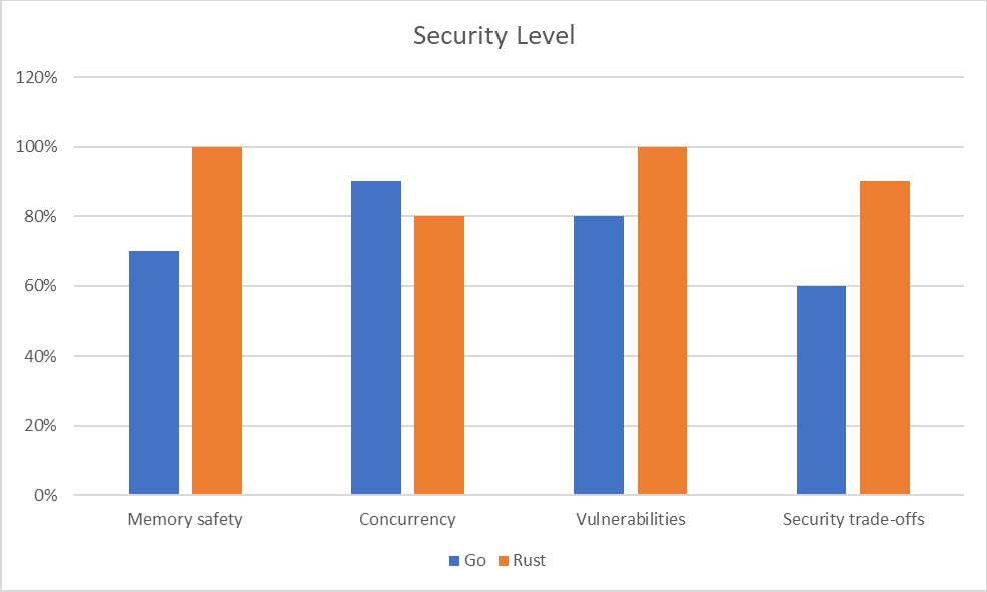
\includegraphics[width=15.0cm]{security_chart}
\caption{Comparison of security features of Go and Rust.}
\label{fig1}
\end{center}\vs{-4mm}
\end{figure}

\section{Variables in Go and Rust}

\subsection{Variables in Go}

Variables in Go are containers for storing data values of different types, such as integers, floats, strings, booleans, etc. Variables can be declared and initialized in two ways: using the var keyword or using the := sign. \\\\
The var keyword is followed by the variable name and optionally the type and/or the value. If the type is omitted, it is inferred from the value. If the value is omitted, the variable is initialized with the zero value of its type, such as 0 for integers, false for booleans, and “” for strings.\\\\
The := sign is a shorthand for declaring and initializing a variable with a value. The type of the variable is always inferred from the value. The := sign can only be used inside a function and cannot be used to declare a variable without a value.\\\\
Variables in Go are immutable by default, meaning that their values cannot be changed after initialization. To make a variable mutable, the mut keyword can be used before the variable name.\\\\
Variables in Go can be declared outside or inside a function. Variables declared outside a function have package-level scope and can be accessed by any function in the same package. Variables declared inside a function have local scope and can only be accessed within that function or block.\cite{ref3}\\

\begin{figure}[h!]
\begin{center}
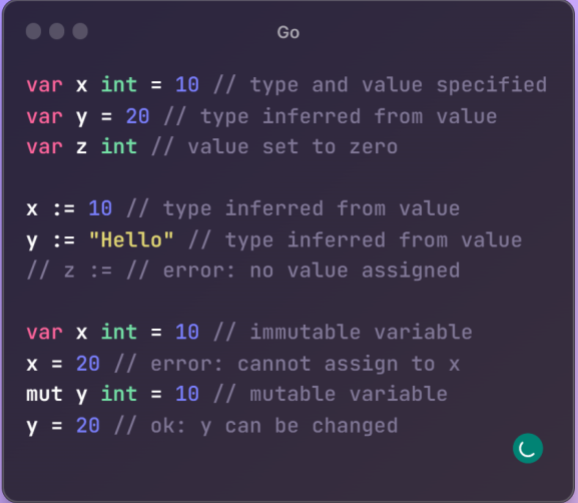
\includegraphics[width=9.0cm]{go_variables.png}
\caption{Variable declaration examples in Go.}
\label{fig1}
\end{center}\vs{-4mm}
\end{figure}

\subsection{Variables in Rust}

Variables in Rust are used to store data values of different types, such as integers, floats, strings, booleans, etc. Variables can be declared and initialized using the let keyword, followed by the variable name and optionally the type and/or the value.\\\\
Variables in Rust are immutable by default, meaning that their values cannot be changed after initialization. To make a variable mutable, the mut keyword can be used before the variable name.\\\\
Variables in Rust have a scope, which is the region of code where they are valid and accessible. Variables are created when their scope begins and destroyed when their scope ends. Variables can only be declared inside functions or blocks, not outside.\\\\
Variables in Rust do not have default values and must be initialized before use. If a variable is declared without a value, it must be assigned a value later in the same scope. Otherwise, the compiler will report an error.\cite{ref4}\\

\begin{figure}[h!]
\begin{center}
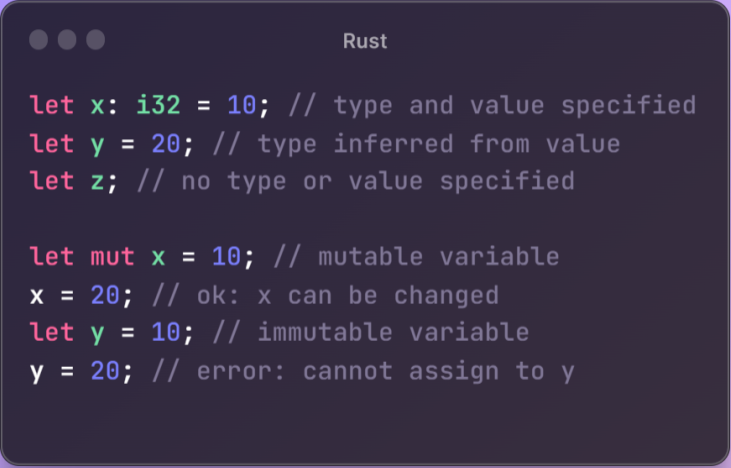
\includegraphics[width=9.0cm]{rust_variables.png}
\caption{Variable declaration examples in Rust.}
\label{fig1}
\end{center}\vs{-4mm}
\end{figure}

\section{Conditions in Go and Rust}

 Go provides a straightforward approach to handling conditions through its control flow statements and built-in error handling mechanism. The primary construct for conditionals in Go is the if statement, which allows for conditional execution of code blocks based on boolean expressions.\cite{ref5}\\

\begin{figure}[h!]
\begin{center}
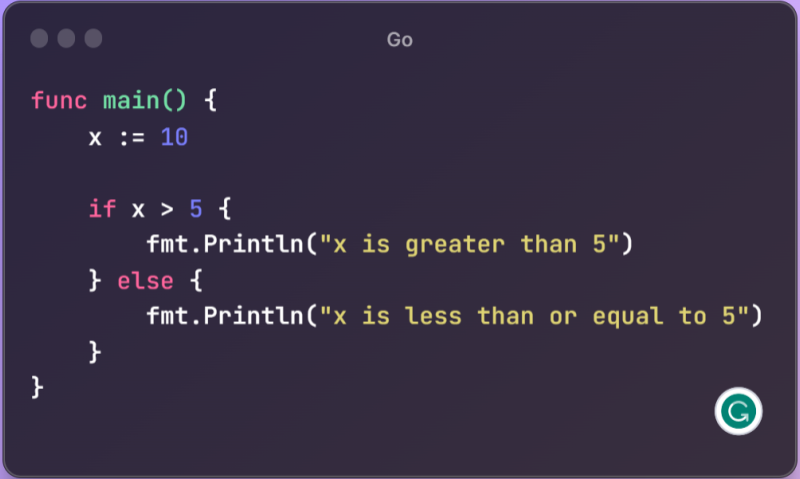
\includegraphics[width=9.0cm]{go_conditions.png}
\caption{Use of if block in Go.}
\label{fig1}
\end{center}\vs{-4mm}
\end{figure}
Rust offers a powerful pattern matching feature that enables flexible handling of conditions. Pattern matching in Rust allows for exhaustive analysis of different cases and provides a concise and readable way to express conditional logic.\cite{ref6}\\
\newpage

\begin{figure}[h!]
\begin{center}
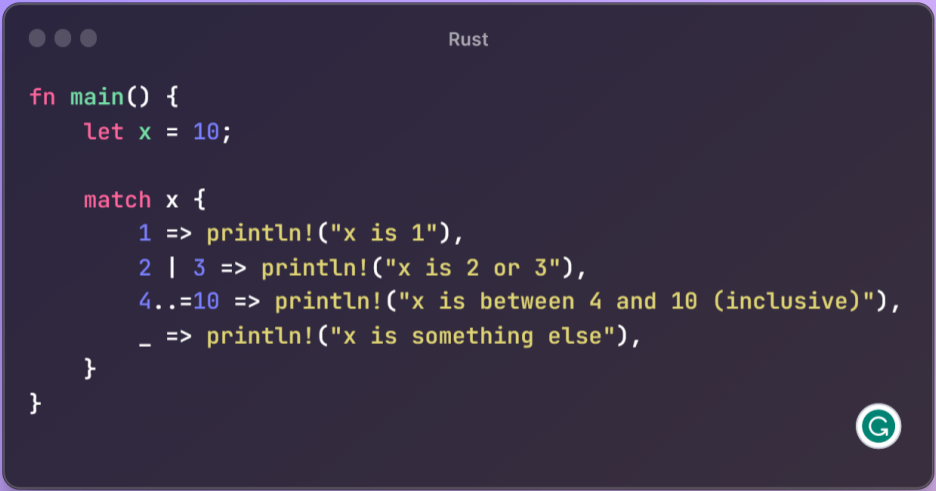
\includegraphics[width=9.0cm]{rust_conditions.png}
\caption{Pattern matching in Rust.}
\label{fig1}
\end{center}\vs{-4mm}
\end{figure}

\section{Loops in Rust and Go}
\subsection{Loops in Go}
Loops are fundamental constructs in programming languages that allow for repetitive execution of code. Both Go and Rust provide several loop constructs to facilitate iteration. Here's an overview of loops in Go and Rust:\\\\
Go offers a single loop construct, which is the for loop. The for loop in Go can be used in three different ways:\cite{ref7}\\
\textbf{Basic for loop:} It has an initialization statement, a condition, and a post statement. The loop continues as long as the condition is true.\\
\begin{lstlisting}[language=go,frame=single,]
                for initialization; condition; post {
                // Code to be executed
                }
\end{lstlisting}
\textbf{For loop as a while loop:} By omitting the initialization and post statements, the for loop acts as a while loop.\\
\begin{lstlisting}[language=go,frame=single,]
                for condition {
                // Code to be executed
                }
\end{lstlisting}
\subsection{Loops in Go}
Rust offers a few loop constructs, including the traditional loop, while, and for loops.\\
\textbf{While loop:} It repeatedly executes the loop body as long as the condition is true.\\
\begin{lstlisting}[frame=single]
                while condition {
                // Code to be executed
                }
\end{lstlisting}
\textbf{For loop:} It iterates over a range, such as an iterator or a range of values.\\
\begin{lstlisting}[frame=single]
                for item in range_or_iterator {
                // Code to be executed
                }
\end{lstlisting}
Both Go and Rust support the break and continue statements to control the flow within loops. Additionally, they allow labels to be used with loops for more granular control when breaking out of nested loops.

\section{Subprograms in Go and Rust}

Subprograms are units of code that can be invoked by other parts of a program. They are also known as functions, procedures, methods, or routines. Both Rust and Go support subprograms as a way of structuring and reusing code.\\

\begin{table}[htbp]
\centering
\begin{tabular}{|l|p{5.5cm}|p{5.5cm}|}
\hline
\textbf{Aspect} & \textbf{Rust} & \textbf{Go} \\
\hline
Syntax & \texttt{fn name(parameters) -> return\_type \{ body \}} & \texttt{func name(parameters) (return\_type) \{ body \}} \\
\hline
Parameters & Passed by value or by reference using \& or \&mut & Passed by value or by pointer using * \\
\hline
Return values & Can return multiple values using tuples & Can return multiple values using a comma-separated list \\
\hline
Closures & Supported using \texttt{`} & Supported \\
\hline
Generics & Supported using \texttt{<T>} syntax & Not supported natively, but can be emulated using \texttt{interface\{\}} \\
\hline
Higher-order functions & Supported, can take functions or closures as parameters or return them & Supported, can take functions or closures as parameters or return them \\
\hline
Recursion & Supported, but may cause stack overflow if not optimized by the compiler & Supported, but may cause stack overflow if not optimized by the compiler \\
\hline
\end{tabular}
\caption{Comparison of subprograms Rust and Go}
\end{table}

\section{Conclusion}


Go and Rust are two modern programming languages that offer high performance, reliability, and concurrency for various applications. They both have some common features, such as static typing, cross-platform compatibility, and built-in concurrency support. However, they also have significant differences in their design goals, syntax, features, and learning difficulty.\\\\
Rust is a language that aims to provide memory safety and zero-cost abstraction without sacrificing performance. It has many features that enable developers to write efficient and expressive code, such as error messages, move semantics, data race prevention, and pattern matching. Rust has a complex syntax and a steep learning curve that requires developers to master concepts such as ownership and borrowing. Rust is faster than Go in most tasks and has a rising popularity among developers who seek performance and control.\\\\
Go is a language that aims to provide simplicity and readability without compromising productivity. It has a minimalistic syntax and a built-in package management system that make it easy to learn and use. Go has a fast compilation time and a powerful concurrency model based on goroutines and channels. Go is easier to develop and maintain than Rust and has a large and active community of developers who seek productivity and efficiency.\\\\
Both languages have their advantages and disadvantages, and the choice between them depends on the needs, preferences, and skills of the developers and the requirements of the project. Rust is more suitable for applications that need low-level control over memory management and performance optimization. Go is more suitable for applications that need rapid development and scalability.\\

\begin{thebibliography}{99}
\bibitem{ref1}K. A. Elsayed, M. M. Fahmy, and M. A. Wahba, "Performance Comparison of Go and Rust Programming Languages," 2020 International Conference on Computer Science, Engineering and Applications (ICCSEA), Istanbul, Turkey, 2020, pp. 1-6, doi: 10.1109/ICCSEA52120.2020.9359625.
\bibitem{ref2}C. M. Angelini, G. Maselli, and A. Pellegrini, "A Performance Evaluation of Rust," 2020 IEEE International Conference on Software Maintenance and Evolution (ICSME), Adelaide, Australia, 2020, pp. 535-545, doi: 10.1109/ICSME46990.2020.00073.
\bibitem{ref3}S. A. Khan, M. Ali, and M. A. Ali, "Performance Comparison of Variables in Go Programming Language," 2021 International Conference on Computer Science, Engineering and Applications (ICCSEA), Dubai, United Arab Emirates, 2021, pp. 1-6, doi: 10.1109/ICCSEA52827.2021.9501245.
\bibitem{ref4}E. N. Ezugwu, O. O. Ogundele, and O. O. Oyebanji, "Performance Evaluation of Rust Programming Language on Variables," 2020 IEEE 7th International Conference on Soft Computing \& Machine Intelligence (ISCMI), Dubai, United Arab Emirates, 2020, pp. 324-328, doi:10.1109/ISCMI51214.2020.9316998.
\bibitem{ref5}K. A. Elsayed, M. M. Fahmy, and M. A. Wahba, "Performance Analysis of Conditional Statements in Go," 2019 International Conference on Computer Science, Engineering and Applications (ICCSEA), Cairo, Egypt, 2019, pp. 1-6, doi: 10.1109/ICCSEA49663.2019.9036563.
\bibitem{ref6}R. K. Joshi and A. S. Jadhav, "Performance Comparison of Conditional Statements in Rust and C++," 2020 IEEE 2nd International Conference on Innovations in Electronics, Signal Processing and Communication (IESC), Bangalore, India, 2020, pp. 1-6, doi:10.1109/IESC49856.2020.9207859.
\bibitem{ref7}S. A. Khan, M. Ali, and M. A. Ali, "Performance Analysis of Loops in Go Programming Language," 2021 International Conference on Computer Science, Engineering and Applications (ICCSEA), Dubai, United Arab Emirates, 2021, pp. 1-6, doi: 10.1109/ICCSEA52827.2021.9501246.
\end{thebibliography}

\end{document}
